	
	 \begin{definition} 
	 	\emph{Главным открытыми множествами} назвают множества вида $D(f) = \AA^n \setminus Z(f)$ для $f \in \Bbbk[x_1, \ldots, x_n]$.
	 \end{definition}

	 Это понятие можно легко перенести на аффинное многообразие. Пусть $X$~--- аффинное многообразие, $\overline{f} \in \cO_{X} = \Bbbk[x_1, \ldots, x_n]/I(X)$, тогда мы можем рассмотреть 
	 \[
	 	D\lr*{\overline{f}} = X \setminus Z\lr*{\overline{f}} = X \cap D(f).
	 \]

	 \begin{remark}
	 	Ясно, что $f = 1 \implies D\lr*{\overline{f}} = X$.
	 \end{remark}

	 Пусть $A = A(X) =  \Bbbk[x_1, \ldots, x_n]/I(X)$~--- координатное кольцо многообразия $X$, мы можем рассмотреть главную локализацию $A_{\overline{f}}$. 

	 Ясно, что у нас есть отображение $A_{\overline{f}} \to \cO_{D(\overline{f})}$. 

	 \begin{remark}
	 	Отметим, что возможен случай, когда $A_{\overline{f}} = 0$, но тогда $\exists k\colon \overline{f}^k = 0$. С другой стороны, так как $I(X)$~--- радикальный идеал, в кольце $A(X)$ нет нильпотентов, то есть $\overline{f} = 0 \implies f \in I \Leftrightarrow D(f) = \varnothing$. В этом случае мы будем принимать соглашение, что $\cO_{\varnothing} = 0$.  	
	 \end{remark}
	 
	 Так вот, отображение $A_{\overline{f}} \to \cO_{D\lr*{\overline{f}}}$ устроено очень просто: 
	 \[
	 	\frac{\overline{a}}{\overline{f}^k} \mapsto \text{ функция } \frac{\overline{a}}{\overline{f}^k}
	 \]
	 Инъективность вполне очевидна:
	 \[
	 	\frac{\overline{a}}{\overline{f}^k}\bigg\vert_{D\lr*{\overline{f}}} = 0 \implies \overline{a}\vert_{D\lr*{\overline{f}}} = 0 \implies \overline{a}\cdot \overline{f}\vert_{X} = 0 \implies af \in I(X) \implies \overline{a} \overline{f} = 0 \in A(X),
	 \]
	 откуда $\overline{a}/\overline{f}^k = 0 \in A_{\overline{f}}$.

	 Докажем теперь сюръективность. Пусть $r \in \cO_{D\lr*{\overline{f}}}$, тогда для $x \in D\lr*{\overline{f}}$ $\exists U_x, \ \overline{g}_x, \overline{h}_x \in A(X)$, где $\overline{h}_x\vert_{U_x} \neq 0$ и $r \overline{h}_x = \overline{g}_x$ на $U_x$ (по определению регулярной функции). 

	 Выбирая многочлен $s_x \in A(X)$, не равный нулю на $U_x$, но обращающийся в ноль на дополнении, мы можем полагать, что наше равенство выполнено на всём $X$. Не умаляя общности, будем считать так изначально. 

	 Рассмотрим идеал $\sum (h_x) + I(X)$ и покажем, что 
	 \[
	   	Z\lr*{\sum_{x \in D\lr*{\overline{f}}} (h_x) + I(X)} \subset Z(f).
	   \]  

	   Действительно, если $y \in  Z\lr*{\sum (h_x) + I(X)}$, то в частности $\forall g \in I(X) \ g(y) = 0 \implies y \in X$, но, $y \notin D\lr*{\overline{f}}$, откуда $y \in Z\lr*{\overline{f}} = X \cap Z(f)$. Отсюда мы получаем, что 
	   \[
	   	\sqrt{(f)} = I\lr*{Z(f)} \subset I\lr*{Z\lr*{\sum_{x \in D\lr*{\overline{f}}} (h_x) + I(X)}} = \sqrt{\sum_{x \in D\lr*{\overline{f}}} (h_x) + I(X)}.
	   \]
	   Отсюда для некотрого $m$ мы имеем $f^m \in \sum_{x \in D\lr*{\overline{f}}} (h_x) + I(X)$, а значит, $\overline{f}^m \in \sum_{x \in D\lr*{\overline{f}}} (\overline{h}_x).$ То есть, у нас есть представление 
	   \[
	   	\overline{f}^m = \sum_{i = 1}^{k} \overline{\ell_{x_{i}}} \overline{h_{x_{i}}} \implies r \cdot \overline{f}^m  = \sum_{i = 1}^{k} \overline{g}_{x_{i}} \overline{\ell_{x_{i}}} \implies r \in A_{\overline{f}}. 
	   \]

	   Таким образом, мы доказали такое предложение 

	   \begin{statement} 
	   	$A_{\overline{f}} \cong \cO_{D\lr*{\overline{f}}}$.
	   \end{statement}

	   Можно доказывать этот факт и иначе. В самом деле, 
	   \[
	   		A_{\overline{f}} \cong A[t]/\lr*{\overline{f}t - 1}.
	   \]
	   Гомоморфизм в обе стороны строится ествественно:
	   \[
	    	\frac{\overline{a}}{\overline{f}^k} \mapsto \overline{a} t^k, \quad t \mapsto \frac{1}{\overline{f}}.
	    \] 
	   \[
	    	A = \Bbbk[x_1, \ldots, x_n]/I(X) \implies A[t]/\lr*{\overline{f}t - 1} \cong \Bbbk[x_1, \ldots, x_n, t]/\lr*{I(x), \overline{f}t - 1},
	    \] 
	    то есть кольцо $A[t]/\lr*{\overline{f}t - 1}$ является координатным кольцом некоторого многообразия $Y$. Это многообразие имеет виде 
	    \[
	    	Y = \{ (x_1, \ldots, x_n, t) \in \AA_{\Bbbk}^{n + 1} \ \vert \ (x_1, \ldots, x_n) \in X, \quad f(x_1, \ldots, x_n) t - 1 = 0 \}. 
	    \]
	    Нарисуем вот такую коммутативную диаграмму:
	    \begin{center}
	    	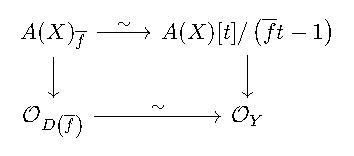
\includegraphics{lectures/5/pictures/pic_1.pdf}
	    \end{center}

	    Горизонтальные стрелки получаются из того, что $Y \xrightarrow{\sim} D\lr*{\overline{f}}$ посредством отображений $(x_1, \ldots, x_n, t) \mapsto (x_1, \ldots, x_n)$ и $(x_1, \ldots, x_n) \mapsto (x_1, \ldots, x_n, 1/f(x_1, \ldots, x_n))$.  Из того, что горизонтальные стрелки~--- изоморфизмы (что нетрудно проверить), вертикальные стрелки также будут изоморфизмами, что нам и нужно. 

	    Поговорим теперь про морфизмы квазиаффинных многообразий. 


	    \begin{statement} 
	    	Пусть $X$~--- квазиаффинное многообразие, $Y \subset \AA^n_{\Bbbk}$~--- аффинное многообразие. Тогда $\psi\colon X \to Y$ является морфизмом в точности тогда и только тогда, когда $x_i \circ \psi$ являются регулярными функциями на $X$ (где $x_i$~--- координатные функции на $\AA^n$).
	    \end{statement}
	    \begin{proof}
	    	В одну сторону утверждение очевидно, докажем в другую. Возьмём замкнутое $T \subset Y$ и проверим, что $\psi^{-1}(T)$ замкнуто. Достаточно проверить это локально, то есть в окрестности любой точки. Возьмём произвольную точку $x \in X$ и докажем, что существует такая окрестность $U_x \ni x$, что $U_x \cap \psi^{-1}(T)$ замкнуто в $U_x$.  Локально отображение $\psi$ можно представить в виде
	    	\[
	    		(x_1, \ldots, x_n) \mapsto \lr*{\frac{f_1(x_1, \ldots, x_n)}{g_1(x_1, \ldots, x_n)}, \ldots, \frac{f_n(x_1, \ldots, x_n)}{g_n(x_1, \ldots, x_n)}}
	    	\]
	    	так как функции $x_i \circ \psi$ регулярны ($x_i$~--- просто проекция на $i$-ю координату) (тут, конечно, для каждой координаты своя окрестность, в которой она представима в таком виде, но все эти окрестности можно и пересечь). 

	    	Не умаляя общности, можно полагать, что $T = \{ y \in Y \ \vert F(y) = 0 \}$ для некотрого полинома $F$. Тогда 
	    	\[
	    		\psi^{-1}(T) \cap U_x = \left\{ (x_1, \ldots, x_n) \bigg\vert F\lr*{\frac{f_1}{g_1}(x_1, \ldots, x_n), \ldots }  = 0 \right\},
	    	\]
	    	откуда $\psi^{-1}(T) \cap U_x$ замкнуто. 

	    	Теперь надо проверить второе условие. Его также можно проверять локально. Возьмём открытое $U \subset Y$ и рассмотрим на нём регулярную функцию $f$. Покажем, что $f \circ \psi$ регулярна на $\psi^{-1}(U)$. Мы можем покрыть $U$ окрестнсотями, на которымх $f$ представляется, как отношение многочленов, пусть $U = \bigcup U_i$ и 
	    	\[
	    		f\vert_{U_i} = \frac{g_i}{h_i}.
	    	\]
	    	Покажем, что $f\vert_{U_i} \circ \psi$ регулярна на $\psi^{-1}\lr*{U_i}$. Соответственно, для этого нам доказать, что композиции $g_i \circ \psi$ и $h_i \circ \psi$ регулярны, а это утверждение очевидно, так как это многочлены от координатных функций. 

	    \end{proof}

	    \begin{remark}
	    	Тут условие аффинности $Y$ не существенно (т.е. это верно и для квазиаффинного). 
	    \end{remark}

	    \begin{statement} 
	    	Пусть $X, Y$~--- многооразия, причем $Y$~--- аффинное. Имеется естественное биективное отображение между 
	    	\[
	    		\Hom_{\qAff}(X, Y) \xrightarrow{\sim} \Hom_{\Bbbk\text{-}\Alg}(A(Y), \cO_{X}).
	    	\]
	    	Естественность тут понимается в естественном смысле: а именно, если у нас есть морфизм $X_1 \to X_2$, то мы получим коммутативную диаграмму:

	    	\begin{center}
	    	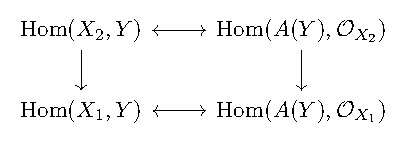
\includegraphics{lectures/5/pictures/pic_2.pdf}
	    \end{center}

	    И, если же у нас есть морфизм $Y_1 \to Y_2$, то мы получим коммутативную диаграмму:  
	    \begin{center}
	    	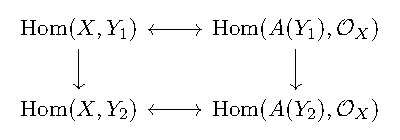
\includegraphics{lectures/5/pictures/pic_3.pdf}
	    \end{center}

	    \end{statement}

	    \begin{proof}
	    	Если у нас есть отображение $X \to Y$, то мы можем построить отображение 
	    	\[
	    		X \to Y \to A(Y) \xrightarrow{\sim} \cO_{Y} \to \cO_{X}.
	    	\]
	    	Посмотрим теперь обратное отобоажение. У нас есть гомоморфзм $h\colon A(Y) \cong \Bbbk[x_1, \ldots, x_n]/I(X) \to \cO_{X}$. Пусть $h(\overline{x_i}) = \xi_i \in \cO_{X}$, тогда мы можем построить отображение $X \to Y$:
	    	\[
	    		X \ni p \mapsto (\xi_1(p), \ldots, \xi_n(p)).
	    	\]
	    	Надо проверить, что мы попадаем именно в $Y$. Возьмём $f \in I(Y)$, надо проверить, что 
	    	\[
	    		f(\xi_1(p), \ldots, \xi_n(p)) = 0.
	    	\]
	    	Заметим, что так как $h$~--- гомоморфизм, 
	    	\[
	    		h\lr*{\underbrace{f\lr*{\overline{x_1}, \ldots, \overline{x_n}}}_{= 0 \text{ в } A(Y)}} = f(\xi_1, \ldots, \xi_n) = 0,
	    	\]
	    	то есть мы действительно попали в $Y$. 

	    	Проверка естественности остаётся читателю в качестве упражнения. 

	    \end{proof}

	    Заметим, что если оба многообразия аффинные, то мы получаем соотвествие 
	    \[
	    	\Hom_{\qAff}(X, Y) \xrightarrow{\sim} \Hom_{\Bbbk\text{-}\Alg}(A(Y), A(X)).
	    \]
	    То есть, мы получаем функтор $\qAff^{op}_{\Bbbk} \to \Bbbk-\Alg$ (где алгебры конечнопорожденные и редуцированные):
	    \[
	    	A\colon \qAff^{op}_{\Bbbk} \to \Bbbk\text{-}\Alg, \quad X \mapsto A(X).
	    \]
	    Кроме того, мы видели, что есть и обратный функтор: если $A \in \Bbbk-\Alg$, то мы можем рассмотреть аффинное многообразие $X'$ такое, что $A(X') \cong A$ и сопоставить $A \to X'$. Этот функтор задан корректно, так как если взять другое многообразие $X$ такое, что $A(X) \cong A(X')$, то изоморфизм алгебр будет индуцировать и изоморфизм многообразий $X \cong X'$ (так как функтор переводит изоморфизмы в изоморфизмы). 

	    Таким образом, мы доказали такую теоремы: 
	    \begin{theorem} 
	    	Категория квазиаффинных многообразий $\qAff$ антиэквивалентна категории конечнопорожденных редуцированных $\Bbbk\text{-}\Alg$ 
	    \end{theorem}

	    \begin{statement} 
	    	Пусть $X$~--- квазиаффиное неприводимое многообразие, $U \subset X$~--- открытое подмножество. Тогда $\dim{U} = \dim{X}$.
	    \end{statement}
	    \begin{proof}
	    	\RNum{1}. Пусть $X$~--- аффинное. Тогда $U = X \setminus Z(f_1, \ldots, f_n) \supset X \setminus Z(\overline{f_1}) = D\lr*{\overline{f_1}}$. то есть, $D\lr*{\overline{f_1}} \subset U \subset X$, откуда 
	    	\[
	    		\dim{D\lr*{\overline{f}}} \le \dim{U} \le \dim{X}. 
	    	\]
	    	Но, поля частных алгебр $A_{\overline{f}}$ и $A$ совпадают, а значит, совпадают и степени трансцендентности, то есть $\dim{D\lr*{\overline{f}}} = \dim{X}$, откуда $\dim{U} = \dim{X}$.

	    	\RNum{2}. Если $X$~-- квазиаффинное, то мы можем вложить его в аффинное: $U \subset X \subset \overline{X}$. $X$ открыто в $\overline{X}$ и 
	    	\[
	    		X = V \cap T = V \cap \overline{X},
	    	\]
	    	откуда $U$ открыто в $\overline{X}$. По пункту $\RNum{1}$ мы получаем $\dim{U} = \dim{\overline{X}}$, а с другой стороны, $X$ открыто в $\overline{X}$, откуда также $\dim{X} = \dim{\overline{X}}$. 
	    \end{proof}

	    \begin{remark}
	    	Пусть $X \subset \AA^m, \ Y \subset \AA^n$~--- аффинные многообразия. Пусть $X = Z(f_1, \ldots, f_k), \ Y = Z(g_1, \ldots, g_{\ell})$, то 
	    	\[
	    		X \times Y = \{ (x_1, \ldots, x_m, y_1, \ldots, y_n) \vert f_i(x_1, \ldots, x_m) = 0, \ g_j(y_1, \ldots, y_n) = 0 \ \forall i, j \}.
	    	\]
	    	То есть, прямое произведение естестенно снабжается структурой аффинного многообразия. Позже мы докажем, что это произведение в категорном смысле. 
	    \end{remark}
	    	

	    \begin{theorem} 
	    	Пусть $Y, Z \subset \AA_{\Bbbk}^n$~--- неприводимые аффинные многообразия, $\dim{Y} = r, \ \dim{Z} = s$. Тогда любая компонента $Y \cap Z$ имеет размерность $\ge r + s - n$.
	    \end{theorem}
	    \begin{proof}
	    	Рассмотрим диагональное вложение 
	    	\[
	    		\Delta\colon \AA^n \to \AA^{n} \times \AA^{n} = \AA^{2n}, \ x \mapsto (x, x). 
	    	\]

	    	Образ $\Delta(\AA^n)$ задаётся нулями многочленов, а значит, замкнут в топологии $\AA^{2n}$. Заметим, что имеет место изоморфизм 
	    	\[
	    		Y \cap Z \xrightarrow{\sim} \Delta\lr*{\AA^n} \cap (Y \times Z).
	    	\]
	    	Так как при изоморфизме неприводимые компоненты переходят в неприводимые компоненты, размерности неприводимых компонент левой и правой частей равны. Чуть позже мы поймём, что 
	    	\[
	    		\dim{Y \times Z} = \dim{X} + \dim{Y}.
	    	\]
	    	Но, по предложению~\ref{dim{X} - m} для размерность лбой компоненты $(Y \times Z) \cap \Delta(\AA^n)$ (но, чтоб им воспользоваться, нужно доказать неприводимость $Y \times Z)$. 

	    	Для завершения доказательства нам надо доказать такой факт: 

	    	\begin{statement} 
	    		Пусть $X \subset \AA^m, \ Y \subset \AA^n$~--- неприводимые аффинные многообразия, то $X \times Y$~--- неприводимое аффинное многообразие в $\AA^{m} \times \AA^{n}$.
	    	\end{statement}
	    	\begin{proof}
	    		Предположми противное, то есть, что 
	    		\[
	    			X \times Y = Z_1 \cup Z_2 \cup \ldots, \quad Z_i \neq X \times Y. 
	    		\]
	    		Ясно, что $\forall x \in X \quad x \times Y \cong Y$ и тоже будет неприводимо. С другой стороны, $x \times Y = ((x \times Y) \cap Z_1) \cup ((x \times Y)\cap Z_1 )$. Тогда по неприводимости мы меем либо $x \times Y \subset Z_1$, либо $x \times Y \subset Z_2$. 

	    		Разобьем все точки на две групы относительно этих условий: 
	    		\[
	    			X = X_1 \cup X_2.
	    		\]
	    		Покажем, что $X_1$ и $X_2$ замкнуты. Их можно представить в таком виде 
	    		\[
	    			X_{1} = \bigcap_{y \in Y} X_{y}, \quad X_{y} = \{ x \in X \vert (x, y) \in Z_1\}
	    		\]
	    		Но, $X_{y}$ замкнуты, так как его можно задать системой уравнений 
	    		\[
	    			\begin{cases} f_1(x, y) = 0, \ldots, f_k(x, y) = 0, \end{cases}
	    		\]
	    		где $f_1, \ldots, f_k$~--- многочлены, задающие $Z_1$.
	    	\end{proof}

	    \end{proof}

    	\begin{exercise}
			Если $X, Y$~--- аффинные, то $A(X \times Y) \cong A(X) \otimes_{\Bbbk} A(Y)$.    
    	\end{exercise}
